\documentclass{article}
\usepackage{graphicx} % Required for inserting images

\usepackage[a4paper, total={6in, 8in}]{geometry}

\usepackage[utf8]{inputenc}
\usepackage[T1]{fontenc}
\usepackage[english]{babel}

\usepackage{amsmath, amssymb, amsfonts}
\usepackage{mathtools}

\usepackage{tikz}
\usetikzlibrary{decorations.pathreplacing,arrows.meta}

\usepackage{amsmath, amssymb, amsthm}



\newcommand{\norm}[1]{\left\lVert#1\right\rVert}
\newcommand{\R}{\mathbb{R}}
\newcommand{\N}{\mathbb{N}}
\newcommand{\Q}{\mathbb{Q}}
\newcommand{\logeq}{\ratio\Leftrightarrow}
\newcommand{\TT}{\Tilde{T}}


\title{Isomorphism between inner product spaces of $\R^n$}
\author{Dias Suleimenov}
\date{April 2024}

\begin{document}

\maketitle

\section*{Introduction}

In usual Linear Algebra course it is not rare task, to calculate coordinates of some vector $y$ relative to basis $U = \{u_1, u_2, ...\}$. If the $U$ is orthogonal basis of $\R^n$, then the formula for calculating coordinates are computationally simple:

\[
([y]_U)_i = \frac{y \cdot u_i}{u_i \cdot u_i}.
\]
Where, $([y]_U)_i$ is i-th coordinate of $y$ relative to basis $U$. 

However, if the basis is not orthogonal, it is required to solve:

\[
[y]_U = U^{-1}y.
\]
Which is unpleasant task to do manually, can't we use another inner product space where the $U$ becomes orthogonal basis and use our simple orthogonal projection formula? In fact we can do it and here is some motivating example.

\subsection*{Motivating Example}

Let \( V = \mathbb{R}^2 \), and take basis vectors:

\[
u_1 = \begin{pmatrix} -1 \\ 1 \end{pmatrix}, \quad u_2 = \begin{pmatrix} 2 \\ 1 \end{pmatrix}.
\]

This basis is \textbf{not orthogonal} with respect to the standard inner product. So, we redefine the inner product as:

\[
\langle u, v \rangle_U := u_1 v_1 + 2 u_2 v_2.
\]

It is easy to check that it is indeed inner product, so it is left to reader. And in this inner product space we have:
\[
\langle u_1, u_2 \rangle_U = (-1)(2) + 2(1)(1) = -2 + 2 = 0,
\]
so \( u_1 \perp_U u_2 \).

\bigskip

Now, for any vector \( y \in V \), we can compute its coordinates in the basis \( U = \{u_1, u_2\} \) using:
\[
[y]_U = \left( \frac{\langle y, u_1 \rangle_U}{\langle u_1, u_1 \rangle_U}, \frac{\langle y, u_2 \rangle_U}{\langle u_2, u_2 \rangle_U} \right).
\]

\subsubsection*{Proof:}

Let
\[
y = \begin{pmatrix} a \\ b \end{pmatrix}, \quad 
C_1 = \frac{\langle y, u_1 \rangle_U}{\langle u_1, u_1 \rangle_U}, \quad 
C_2 = \frac{\langle y, u_2 \rangle_U}{\langle u_2, u_2 \rangle_U}.
\]

We compute:
\[
\langle u_1, u_1 \rangle_U = (-1)^2 + 2(1)^2 = 3, \quad
\langle y, u_1 \rangle_U = (-1)(a) + 2(b) = -a + 2b,
\]
\[
\Rightarrow C_1 = \frac{2b - a}{3}.
\]

Also,
\[
\langle u_2, u_2 \rangle_U = 2^2 + 2(1)^2 = 4 + 2 = 6, \quad
\langle y, u_2 \rangle_U = 2a + 2b = 2a + 2b,
\]
\[
\Rightarrow C_2 = \frac{2a + 2b}{6} = \frac{a + b}{3}.
\]

Now verify the decomposition:
\[
U[y]_U = C_1 u_1 + C_2 u_2 = 
\frac{-a + 2b}{3} \begin{pmatrix} -1 \\ 1 \end{pmatrix} 
+ \frac{a + b}{3} \begin{pmatrix} 2 \\ 1 \end{pmatrix}
= \begin{pmatrix} a \\ b \end{pmatrix}.
\]

So \( C_1, C_2 \) are indeed the coordinates of \( y \) relative to basis \( U \). \qed

\bigskip

After motivating example, it is tempting to generalize further, to make any basis of \( \R^n \) orthogonal. So we proceed with generalization.

\section*{Orthogonalization via Inner Product Construction}

Suppose we have a basis \( u_1, \ldots, u_n \in \mathbb{R}^n \). Is it possible to define an inner product such that \( u_1, \ldots, u_n \) become orthogonal? Apparently, yes --- with the following construction:

Define:
\[
  \langle x, y \rangle :=  (A^{-1}x) \cdot (A^{-1}y) = (A^{-1}x)^T (A^{-1}y) = x (A^{-1})^T(A^{-1})y, \quad \text{where } A = [u_1\,\cdots\,u_n].
\]

We verify the four inner product axioms:

\begin{enumerate}
  \item \textbf{Symmetry:}
  \[
  \langle x, y \rangle = (A^{-1}x)^T (A^{-1}y) = (A^{-1}y)^T (A^{-1}x) = \langle y, x \rangle.
  \]

  \item \textbf{Linearity in the first argument:}
  \[
  \langle u+v, w \rangle = (A^{-1}(u+v))^T A^{-1}w = (A^{-1}u + A^{-1}v)^T A^{-1}w = \langle u, w \rangle + \langle v, w \rangle.
  \]

  \item \textbf{Homogeneity:}
  \[
  \langle cu, w \rangle = (A^{-1}(cu))^T A^{-1}w = c (A^{-1}u)^T A^{-1}w = c \langle u, w \rangle.
  \]

  \item \textbf{Positive Definiteness:}
  \[
  \langle x, x \rangle = (A^{-1}x)^T (A^{-1}x) = \|A^{-1}x\|^2 > 0 \quad \text{for } x \ne 0.
  \]
  Since \( A \) is invertible, \( A^{-1}x = 0 \Rightarrow x = 0 \).
\end{enumerate}

Now we proceed that under such construction basis $U$ becomes orthogonal and orthogonal decomposition in such inner product space works.

\subsection*{Orthogonality of Basis}

To show that \( u_i \perp u_j \) for \( i \ne j \), compute:
\[
\langle u_i, u_j \rangle = (A^{-1}u_i)^T (A^{-1}u_j) = e_i^T e_j = 0.
\]
This holds since \( A^{-1}u_i = e_i \), the standard basis vector.

\subsection*{Orthogonal Decomposition}

Let \( y \in \mathbb{R}^n \). Then we can decompose:
\[
y = \sum_{i=1}^n \frac{\langle y, u_i \rangle}{\langle u_i, u_i \rangle} u_i.
\]

We verify:
\begin{align*}
  \sum_{i=1}^n \frac{\langle y, u_i \rangle}{\langle u_i, u_i \rangle} u_i
  &= \sum_{i=1}^n \left( \frac{(A^{-1}y)^T e_i}{e_i^T e_i} \right) u_i \\
  &= \sum_{i=1}^n ((A^{-1}y)^T e_i) u_i \\
  &= A (A^{-1} y) = y.
\end{align*}

Hence, even though the basis is not orthogonal under the standard dot product, we can define an inner product under which it is orthogonal and still retain decomposition. \qed

\bigskip

Our construction gave us huge class of inner products. Natural question to ask, whether all inner product of $\R^n$ have such form or not? Interestingly all inner products are actually of such form. And here is proof.

\section*{Isomorphism between inner product spaces of $\R^n$}

Let \( U = [u_1, \dots, u_n] \), where \( u_1, \dots, u_n \) is an orthonormal basis with respect to the inner product \( \langle \cdot, \cdot \rangle \). Such a basis exists via Gram–Schmidt orthonormalization process. It is classical result, so proof omitted.

Let \( x, y \in \mathbb{R}^n \). Then, since \( u_1, \dots, u_n \) is a basis,
\[
x = \alpha_1 u_1 + \cdots + \alpha_n u_n, \quad y = \beta_1 u_1 + \cdots + \beta_n u_n, \quad \text{for some } \alpha_i, \beta_i \in \mathbb{R}.
\]

Then:
\begin{align*}
\langle x, y \rangle &= \left\langle \sum_{i=1}^n \alpha_i u_i,\; \sum_{j=1}^n \beta_j u_j \right\rangle \\
&= \sum_{i,j} \alpha_i \beta_j \langle u_i, u_j \rangle \\
&= \sum_{i=1}^n \alpha_i \beta_i \quad \text{(since \( u_i \perp u_j \) for \( i \ne j \), and \( \|u_i\| = 1 \))}.
\end{align*}

On the other hand, since \( U^{-1} x = (\alpha_1, \dots, \alpha_n)^T \), and \( U^{-1} y = (\beta_1, \dots, \beta_n)^T \), we have:
\[
(U^{-1} x)^T (U^{-1} y) = \sum_{i=1}^n \alpha_i \beta_i.
\]

Therefore,
\[
\langle x, y \rangle = (U^{-1} x)^T (U^{-1} y).
\] \qed

Intuitive interpretation of this result is that -- any inner product space \( \mathbb{R}^n \) is isomorphic to standard Euclidean space, under a change of basis. The inner product is essentially the dot product in transformed coordinates. Such visualization can aid intuitive understanding:

\bigskip 

As before, let
\[
u_1 = \begin{pmatrix}-1\\1\end{pmatrix},\quad
u_2=\begin{pmatrix}2\\1\end{pmatrix},\quad
A=[\,u_1\;u_2\,].
\]
Under the new inner product \(\langle x,y\rangle=(A^{-1}x)^\top(A^{-1}y)\), the skewed axes \(u_1,u_2\) become orthonormal.  Here’s how the integer grid in the standard coordinates  
\(\{(i,j):i,j\in\mathbb Z\}\)  
gets mapped by \(A\):


\bigskip
\begin{center}
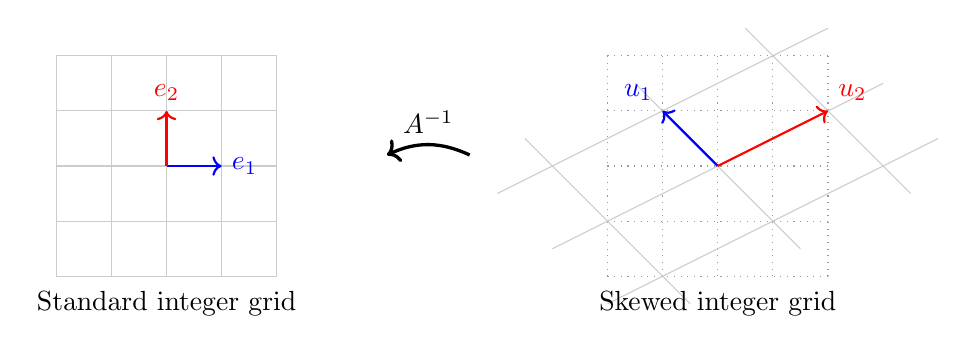
\begin{tikzpicture}[scale=0.7]
  % Left: standard grid
  \begin{scope}
    \foreach \i in {-2,-1,...,2} {
      \draw[gray!40] (\i,-2) -- (\i,2);
      \draw[gray!40] (-2,\i) -- (2,\i);
    }
    \draw[thick,->,blue] (0,0) -- (1,0) node[right] {$e_1$};
    \draw[thick,->,red] (0,0) -- (0,1) node[above] {$e_2$};
    \node at (0,-2.5) {Standard integer grid};
  \end{scope}

  % Curved arrow
  \draw[very thick,<-,bend left=25] (4,0.2) to node[midway,above] {$A^{-1}$} (5.5,0.2);

  % Right: transformed grid
  \begin{scope}[xshift=10cm]
    % faint original grid background
    \foreach \i in {-2,-1,...,2} {
      \draw[dotted,gray!80] (\i,-2) -- (\i,2);
      \draw[dotted,gray!80] (-2,\i) -- (2,\i);
    }
    % transformed vertical lines
    \foreach \j in {-1,0,1} {
      \draw[gray!40]
        plot[domain=-1.5:1.5,samples=2]
        ({2*\x - \j}, {\x + \j});
    }
    % transformed horizontal lines
    \foreach \i in {-1,0,1} {
      \draw[gray!40]
        plot[domain=-1.5:1.5,samples=2]
        ({2*\i - \x}, {\i + \x});
    }
    % axes u1, u2
    \draw[thick,->,blue] (0,0) -- (-1,1) node[above left] {$u_1$};
    \draw[thick,->,red]  (0,0) -- (2,1)  node[above right]{$u_2$};
    \node at (0,-2.5) {Skewed integer grid};
  \end{scope}
\end{tikzpicture}
\end{center}

Under this mapping, each square cell becomes a parallelogram spanned by \(u_1\) and \(u_2\).
In the new inner product, those axes behave exactly like standard orthonormal axes under the dot product.
\end{document}